\chapter{Analyses}%%%%%%%%%%%%%%%%%%%%%%%%%%%%%%%%%%%%%%%%%%%%%% 
\label{chap:analyses}

\begin{note}
  better answering questions at the end, not throughout the thesis
\end{note}

In this chapter the various software implementations and design choices made in \refchap{chap:implementation} are analyzed. 
First, \refsec{sec:analyses:representation}.
Second, \refsec{sec:analyses:compilation}.
Then, \refsec{sec:analyses:loading}.
Finally, \refsec{sec:analyses:utilization}.

\section{The base application}
\label{sec:analyses:representation}

This section of the analysis covers the question of \mySubRQOneTitle, and aims in particular to answer the questions: \emph{Per requirement, to what extent is it successfully implemented by this dataflow-VPL?} and \emph{Per requirement, which role did the core browser features play in supporting or hindering it?}.

Additionally, this section clarifies to what extent a feature could not be implemented due to shortcomings of this particular implementation, or due to a limitation of the browser environment as a whole. 

% We group the requirements listed at \refsec{sec:method-one} in a group of base features,
% a group of dataflow features, and a group of geometry features.

\subsection*{The extent of the dataflow-VPL implementation}

\refsec{sec:method-one} named the following features which had to be implemented:
\begin{enumerate}[-]
  \item a base 'programming language model'
  \subitem A representation of the 'variables' and 'functions' of the language
  \subitem With all computations being pure functions
  \subitem With all variables being immutable
  \item a 'graph-like' visualization of this data model
  \item an interface to create and edit this graph 
  \item a way to provide input data 
  \item a way to execute the language
  \item a way to display or save output data
\end{enumerate}

\subsubsection*{The model}
A basic (visual) programming language model was able to be fully implemented on the web. 
No special web features were utilized in the creation of this model, despite HashMaps and HashSets offered by the Typescript language. 

\subsubsection*{Visualization}
Visualization of the graph is implemented using the 2D canvas api.  
On every registered change to the graph, the canvas is redrawn. 
The 2D canvas api makes use of explicit draw calls, rather than 'defining' some visualization, and leaving the render sequence to the renderer itself, like HTML.
This way, One does not have to first 'create' a circle object and pass it to a renderer. 
A circle can instantly and directly be drawn at the position specified.
The downside of this implementation, is that all features the HTML renderer normally accounts for, like picking, conditional styling, and performant rendering of repetitious elements, are lost.
These have to be re-implemented in javascript, which will never be as performant as the codebase of the browser engines themselves. 
This makes the visualization slow while rendering a large amount of components (See TODO). 

\begin{note}
  TODO Show a graph with performance considerations
\end{note}

This slowness can be blamed partially on the implementation, and partially on the browser. 
The browser does not offer the 'middle ground' between html-like rendering and 2D canvas-like rendering required for a visualization like the dataflow graph. 
Still, this implementation could have experimented more with a HTML + SVG based render method.

\subsubsection*{Editing}
Editing of the graph was made possible by the various events offered by the browser api. 
This allows the graph to be editable using the mouse. 
The graph even offers 'undo' and 'redo' operations, and even 'copy' / 'paste' clipboard actions, using common shortcuts. 
However, the implementation does lack touch \& mobile support.

In general, these editing features are complete, but there are a few caveats caused by the browser environment.
Namely, the browser has need of its own controls and shortcuts. 
For example, the right mouse button brings up the browser context, and the \m{Ctrl + W} shortcut closes a browser tab, which cannot be overwritten.
While there are some workarounds, these aspects make web applications more 'convoluted' to implement than would otherwise be ideal.

\subsubsection*{Execution}
Execution of the graph works as described, albeit with a major setback: execution does not run on a separate thread. 
This means that the interface freezes up during large calculations, and this is not acceptable. 

The reason for this is the difficulty in achieving concurrency in the browser. 
To create a thread, one has to instantiate a so called 'web worker' \emph{with} the actual source code included in a parameter. 
Not only is this unusual, it forces a codebase to create separate files per thread.
The dynamic nature in which some of Geofront dependencies are loaded made splitting up the codebase like this impossible, let alone using multiple threads for calculating each node.

\subsubsection*{Input and Output}
The base dataflow VPl component of Geofront support input and output UI elements, like sliders, buttons, and text fields.
These form special nodes on the canvas, called 'widgets'. 
The fact that the Geofront implementation opted for a 2D canvas-based visualization made it so HTML could not be used for these aspects, and all these features had to be created from scratch.


%%%%%%%%%%%%%%%%%%%%%%%%%%%%%%%%%%%%%%%%%%%%%%%%%%%%%%%%%%%%%%%

\subsection*{The extent of the geometry support implementation}

\refsec{sec:method-one} named the following features as a requirement for geometry support:
\begin{enumerate}[-]
  \item Type safety 
  \item A way to load or to create geometry data 
  \item A way to export geometry data
  \item A method to preview geometry data in 3D
  \item A standard set of geometric types and operations
\end{enumerate}

\subsubsection*{Type Safety}
Type safety was fully implemented by essentially creating a new 'layer' of types in typescript.
The type system can be extended by types found in Geofront Plugins.  
In theory, this can be used to prevent all incorrect type usage during creation of a Geofront Script.
In practice, to support iteration, some runtime type checking was still required. 

\subsubsection*{IO}
Files can be used as inputs and extracted as outputs using the 'file load' and 'file save' widgets. 
These files are then loaded as raw text or raw binary, which can be parsed by using a parser appropriate for that file type. 
The problem with this implementation, is that it requires a full file to be loaded into memory. 
Most native parsers make use of streaming to avoid this. 
There are ways of supporting incrementally reading files in a browser, but these methods are not supported by all browsers yet. 

\subsubsection*{Visualization}
Visualization of 3d data used throughout the graph is possible thanks to WebGL. 
The useful aspect of WebGL is the fact it does not have to be included within the source code of a program. 
WebGL supports all render demands basic, small-scale 3D geodata visualization might need, such as point clouds and DTMs.
large scale visualization is not possible, as the visualizer does not support idioms like frustum culling, or dynamic levels of detail. 

\subsubsection*{Standard Geometry \& Operations}
lastly, the browser and this implementation were able to support the models and operations required for basic 3D geometry, like points, lines, polygons, and meshes.
the "TypedArray" browser feature is used extensively to bypass the fact that javascript has limited type support.

%%%%%%%%%%%%%%%%%%%%%%%%%%%%%%%%%%%%%%%%%%%%%%%%%%%%%%%%%%%%%%%%%%%%%%%%%%%%%%%
%%%%%%%%%%%%%%%%%%%%%%%%%%%%%%%%%%%%%%%%%%%%%%%%%%%%%%%%%%%%%%%%%%%%%%%%%%%%%%%
%%%%%%%%%%%%%%%%%%%%%%%%%%%%%%%%%%%%%%%%%%%%%%%%%%%%%%%%%%%%%%%%%%%%%%%%%%%%%%%
%%%%%%%%%%%%%%%%%%%%%%%%%%%%%%%%%%%%%%%%%%%%%%%%%%%%%%%%%%%%%%%%%%%%%%%%%%%%%%%
%%%%%%%%%%%%%%%%%%%%%%%%%%%%%%%%%%%%%%%%%%%%%%%%%%%%%%%%%%%%%%%%%%%%%%%%%%%%%%%
%%%%%%%%%%%%%%%%%%%%%%%%%%%%%%%%%%%%%%%%%%%%%%%%%%%%%%%%%%%%%%%%%%%%%%%%%%%%%%%
%%%%%%%%%%%%%%%%%%%%%%%%%%%%%%%%%%%%%%%%%%%%%%%%%%%%%%%%%%%%%%%%%%%%%%%%%%%%%%%
%%%%%%%%%%%%%%%%%%%%%%%%%%%%%%%%%%%%%%%%%%%%%%%%%%%%%%%%%%%%%%%%%%%%%%%%%%%%%%%
%%%%%%%%%%%%%%%%%%%%%%%%%%%%%%%%%%%%%%%%%%%%%%%%%%%%%%%%%%%%%%%%%%%%%%%%%%%%%%%

\section{Compilation Process}
\label{sec:analyses:compilation}

\subsection{First part}

\begin{note}
[Show the performance benchmarks in isolation. Also show them in action on the VPL canvas]
\end{note}
  
\subsection{Second part}


\begin{note}

  REQUIREMENT: libraries containing pure functions exclusively
  - no side effects, thats the whole point
  
  
  HOWEVER 
  - existing geo-libs: 
    - file IO focussed, (because of streaming \& big data)
    - templates
    - 
  
  [Analyze the web-exposed geoprocessing libraries]
  
  
  The catch 21 between C++ and Rust.  

  **C++ -> wasm is difficult**
  
  - requires a lot of trivia knowledge. 
    - Often, many subdependencies need to be traversed, and makefiles need to be manually edited. 
    - This cannot be done often, or easely. 
  - Documentation is behind compared to Rust.

  - Libraries cannot be called. emscripten prefers a cli-type interface, and prefers you to write all the operations you wish to publish as separate command line applications. 

  https://www.hellorust.com/demos/add/index.html
  https://emscripten.org/docs/porting/connecting_cpp_and_javascript/embind.html


  **rust-> wasm is powerful and feature-rich.** 
  
  - it functions like a normal compiler. compilation was done easely. 
  - If a library cannot be compiled, the compiler statements are clear enough to identify which library causes the incompatibility. 
  - Many Rust libraries also conveniently offer a 'no-std' option, 
    And many crates (Rust equivalent of a library) include the web as one of their core targets. 
  - The compile tool 'wasm-bindgen' has excelent support for converting libraries. 
    - You can create rust libraries which from the outside look like a normal javascript library. 


    - figure out the difference in load time and performance between startin's tin, cgal's tin, and my dumb triangulator.

\end{note}

\begin{note}
  where C++ requires emscripten, rust does that almost out of the box, (rustup target add wasm32-unknown-unknown), NOTE C++ also does that with CLANG and LLVM

  What we actually need to compare is not emscripten and wasm-bindgen, but 'embind' and 'wasm-bindgen'. 
\end{note}

\section{Loading plugins}
\label{sec:analyses:loading}

In this section is meant to assess to what extent Geofront's plugin loader mitigates the need for explicit configuration.
This analysis is based on the achievements and limitations explained by \refsec{sec:implementation:loading}.

\subsection*{To what extent does the plugin loader mitigate the need for explicit configuration of plugin libraries?}

Based on the results, we can state that the loader mitigates the need for explicit configuration only for the required, mandatory aspects. 
All optional properties like human-readable names and descriptions, must be specified explicitly using a naming convention specific to Geofront. 

In practice, however, there are some more "configuration" requirements. 
The limitations outlined by \refsec{sec:implementation:loading:limits} show that there are quite a few additional considerations. 
Geofront does not support all types or all library structures, and certain languages require additional compile limitations.

Also, while the optional properties are, well, optional, one could argue that some of these properties are in fact required. 
Libraries without 'human-readable' names and descriptions are harder to utilize on the Geofront Canvas.
While regular programming languages also allow the creation and publication of undocumented libraries, one can question if this should also be allowed for the more end-user focussed VPL libraries.

So, while the plugin loader can load some simple textual programming libraries almost without any special configuration, sizable libraries intended for consumption by Geofront will still need to be explicitly configured for Geofront.
However, even with these requirements, this can still be considered an improvement compared to the plugin systems of geometry VPLS studied at \refsec{sec:related-geovpl}, 
in which developers are required to create a class per exposed function.

\subsection*{Assess to what extent this creates seamless interoperability between textual programming libraries, and VPL libraries?}

Because of the reasons outlined above, it is safe to say that this seamless interoperability is only one-directional: Libraries intended for consumption by Geofront double as also a 'normal' javascript library. 
The configuration demands of Geofront only impair the normal, javascript-based usage by forcing a functional style, and by including certain methods only intended for Geofront. 
Even these Geofront-specific methods might prove useful in certain scenarios, such as by providing a way to visualize data.

This seamless interoperability is less prominent in the opposite direction. 
A normal javascript library, or a javascript library using WebAssembly, can't be automatically used by Geofront in most cases. 
Most libraries use incompatible types, or have an incompatible architecture.
In some cases, a library might be able to load, but is then functionality impaired by the interface. 
\reffig{fig:oop-considered-harmful} is an example of such a case.

\begin{figure}
  \centering
  \graphicspath{ {../../assets/images/6/3/} }
  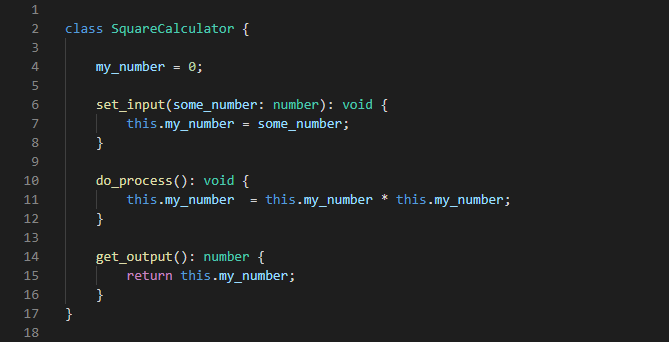
\includegraphics[width=\linewidth]{ugly-oop.png}
  \caption[]{This typescript file technically loads correctly into Geofront, but cannot be reasonably used on the Geofront canvas. TODO: show what this looks like on canvas}
  \label{fig:oop-considered-harmful}
\end{figure}

\section{Usability}
\label{sec:analyses:utilization}

This section offers an analysis on the usability of Geofront, according to the framework described by \cite[]{green_usability_1996}.

Abstraction gradient: What are the minimum and maximum levels of abstraction? Can fragments be encapsulated

\subsection*{Abstraction gradient: What are the minimum and maximum levels of abstraction? Can fragments be encapsulated?}

Geofront was meant to support encapsulation. 
The need for re-using parts of a script as components / functions was deemed more important than the benefits of having no abstraction hierarchy (what you see is what you get).
An early prototype of Geofront did allow for encapsulation, by taking a subset of a Geofront script, and compiling it to a javascript subset. This could then be loaded by the library loader. 
However, the addition of special types of nodes, and features like iteration, invalidated the \m{geofront -> js} translator.
The translation is still possible, just not implemented.  
As such, if a user desires re-usable components and a lower abstraction level, they will need to write a Geofront library.

\textbf{Suggestion for improvement:} re-implemented the 'compile to js' procedure.

(image of abstracting away a javascript subset)



\subsection*{Closeness of mapping: What 'programming games' need to be learned?}

Mapping a problem to a geofront script is intuitive for the most part.
Think of the operations needed to solve a problem, 
find the right libraries and nodes representing these operations,
and connect these nodes according to type. 
However, this mapping of problem and solution is hindered by the fact that Geofront needed to support iteration. 

(image of iteration problem)



\subsection*{Consistency: When some of the language has been learnt, how much of the rest can be inferred?}

\cite[]{green_usability_1996} notes on the difficulty of defining 'consistency' in language design, and chose to define it as a form of 'guessability'.

Geofront has introduced certain symbolic distinctions between graphical entities to aid this predictability. 
The biggest is the distinction between \m{operation} and \m{widget} components: 
operations are pure functions with inputs and outputs. 
widgets represent some 'outside world' interaction, like an input value, a file, or a web service. 
This way, 'special behavior' is isolated to widgets, making the rest of the script more predictable. 

In practice, certain inconsistencies within Geofront arise due to the open nature of the plugin system. 
the consistency of geofront is mitigated by a library with a very different notion of naming, or if the library chooses unusual input or output patterns. 
For example, a euclidean, 3D coordinate can be specified as a \m{Vector3} object, a struct, an array of three numbers, or three different x, y, z input parameters.
Then again, it is unclear if inconsistencies between the api's of a language's libraries are to be contributed to the inconsistency of the language as a whole. 

\textbf{Suggestion for improvement:} Stabilize the api of the Geofront Standard Library.



\subsection*{Diffuseness: How many symbols or graphic entities are required to express a meaning?}

Geofront periodically suffers from the same 'Diffuseness' problems \cite[]{green_usability_1996} adheres to vpls general. 
That is, sometimes a surprising number of 'graphical entities' / nodes are required to represent a simple statement.  
This is apparent when representing mathematical calculations. 

\begin{note}
  - the flowchart can only represent linear processes. Many geoprocessing algorithms are iterative and make use of conditionals. These cannot easily be expressed in a DAG VPL. As such, these processes must happen within the context of a function, within a 'computational node'  
\end{note}


(image of complex / simple mathematical calcluation in javascript and in geofront)

\textbf{Suggestion for improvement:} These situations could be prevented by allowing scriptable components. 

\subsection*{Error- proneness: Does the design of the notation induce 'careless mistakes'?}

There are some errors the user can make  in Geofront that will not be immediately obvious. 
The biggest one is that there are no systems in place preventing large calculations. 
These might freeze up the application. 

To prevent this, the geofront interpreter should have been implemented to run on a separate thread, using a web worker. 
Besides this, in general, many systems are in place preventing errors, such as the type-safety used throughout geofront.
Also, by disallowing cyclical graphs, users cannot create infinite loops accidentally.

\subsection*{Hard mental operations: Are there places where the user needs to resort to fingers or pencilled annotation to keep track of what's happening?}

Geofront is developed specifically to prevent "Hard mental operations".
Following the dataflow paradigm explained in \refsec{sec:background:dataflow}, geofront chose to disallows cyclical patterns. 
This greatly reduces the complexity of possible graph configurations, and also causes all in-between results to be immutable or 'final'.
By then allowing these results to be inspected, and allowing the graph to be easily reconfigured, Geofront allows a workflow rooted in experimentation and 'play'.
Users do not need to 'keep track' or 'guess' how things work.
Instead, they can simply experience the behavior, and adjust the behavior until satisfied. 



\subsection*{Hidden dependencies: Is every dependency overtly indicated in both directions? Is the indication perceptual or only symbolic?}

The dimension of 'hidden dependencies' is another way the dataflow-paradigm is advantageous. 
The pure functions of a diagram-based vpl like Geofront make the language in general consistent and predictable.
However, there are two exceptions to this rule:
First, the \m{widget} nodes are allowed to produce side-effects, such as opening a window, asking for an input, making a web request, etc. 
These are required to provide geofront with interactive inputs and outputs.
The distinction between \m{widgets} and \m{}

And second, the pureness of functions can only be maintained if all Geofront libraries also exclusively use pure functions. 
There is no fail-safe in place to prevent the usage of a library containing functions with many side-effects. 

\subsection*{Premature commitment: Do programmers have to make decisions before they have the information they need?}

In general, Geofront requires almost no premature commitment. 
Or, rather, the level of premature commitment is in line with textual programming languages, in the sense that a user is always somewhat committed to the structure they themselves build. 

One practical way in which Geofront exceeds in this dimension of premature commitment, is that the application does not require a restart upon loading a new library. 
Users can add or remove libraries "on the fly". 
This is unlike any vpl studied at \refsec{sec:related-geovpl} or \refsec{sec:related-webvpl}.

One particular type of commitment users must be aware off, however, is the commitment to using a \ac{vpl} like Geofront. 
Therefore, 


\subsection*{Progressive evaluation: Can a partially-complete program be executed to obtain feedback on 'How am I doing'?}

Yes. 
As explained at the answer for the dimension of 'Hard mental operations', this is a core aspect in how Geofront achieves its interactivity and debugability, together with its ability to inspect parameters. 

(Image: Show example)

\subsection*{Role- expressiveness: Can the reader see how each component of a program relates to the whole?}

as the authors of \cite[]{green_usability_1996} write: "The dimension of role-expressiveness is intended to describe how easy it is to answer the question 'what is this bit for?'"

sizeable phenomenon

grootste boosdoener: looping is now a simple boolean toggle within a component. 
This makes it very non-explicit, 

This leads to another problem: the problem of declarative iterations within a vpl. 


\subsection*{Secondary notation: Can programmers use layout, color, other cues to convey extra meaning, above and beyond the 'official' semantics of the language?}

No, Geofront does not offer annotations in its current state, besides the way the nodes are configured on the canvas.  
Geofront does provide visual indicators for types, and for if a cable / variable represents a single item, or a list of items.

\textbf{Suggestion for improvement:} Provide a way to annotate: create groups, write comments, etc. 
\textbf{Suggestion for improvement:} Type colors would also be nice.

\subsection*{Viscosity: How much effort is required to perform a single change?}

Despite these efforts, the 'mouse intensive' interface of vpls like Geofront continues to be a hinder for viscosity.
Certain situations require excessive mouse interaction, like substituting a function with another function, but keeping all inputs the same.
In text, this would be as simple as a non-symbolic renaming of the called function.
In geofront, this requires a lot of reconfiguration of cables. 

\textbf{Suggestion for improvement:} Viscosity could be improved by creating special actions in the editor to perform these types of manipulations.  
%  - select multiple inputs, select multiple outputs: connect by height.
% rename node


\subsection*{Visibility: Is every part of the code simultaneously visible (assuming a large enough display), or it it at least possible to juxtapose any two parts side-by-side at will? If the code is dispersed, is it at least possible to know in what order to read it?}

All parts of the code are simultaneously visible. 
As the question implies, by not making the code dispersed, 

% ## Case Studies

% ### Vector
% _Vector data retrieval, transformation, visualization_

% ### Raster 
% _Raster data retrieval, transformation, visualization_

% ### 6. Experiments 
% _Performance benchmark between rust-wasm / cpp-wasm / cgal-cpp-wasm / js / cli usage_

% ## Final 
% _Answer research questions ????_


% \section{Experiments}

% \subsection{ Web Mapping Service }
% -> could work, must be captured in component
% -> streaming question

% \subsection{ Open Street Map }
% -> could be hooked up to the geojson viewer



% \section{ Performance }
% \subsection{Vector 3D}

% ....

% \subsection{Raster}

% ....

% \subsection{Geo features}

% ....


%%%%%%%%%%%%%%%%%%%%%%%%%%%%%%%%%%%%%%%%%%%%%%%%%%%%%%%%%%%%%%%%%%%%%%%%%
% \section{Use Case: Educational Sandbox}
% \begin{lstlisting}
% WHAT: 
%  - show the behaviour of a simple ransac algorithm, fitting a plane through 
%    a point cloud
%  - show it beharivourly: show in-between steps
%  - make parameters ajustable (number of high scores, minimum high score, 
%    number of tries, etc.)
%  - add least squares adjustment, and compare.

% SIMILAR EXAMPLES: 
%  - the geometric predicates explanation 
%  (https://observablehq.com/@mourner/non-robust-arithmetic-as-art)
%  - 

% ASSESS ON: 
%  - educational value
%  - ease of usage (the promise of **Criterium A**)
 
% ASSESSMENT (hypothesis): 
%  + indeed very insightful for analying the behaviour 
%    and operation of certain 
%    algorithms & parameters. Not many applications can show 
%    this level of insight. 
%  + feature B can be used to strip the tool down 
%    to the bare minimum,   helping 
%    with not overwhelming the user with features

%  - This VPL is not easy to operate. 
%    It remains difficult to communicate what needs to 
%    be done, how things work. This is not an expert tool, 
%    but also not a beginners' tool.
%  - No built-in tutorialization
%  - hard to discover the code underneath, 
%    obfuscating the link between process and code.

% \end{lstlisting}

% %%%%%%%%%%%%%%%%%%%%%%%%%%%%%%%%%%%%%%%%%%%%%%%%%%%%%%%%%%%%%%%%%%%%%%%%%
% \section{Use Case: Web Demo Environment}
% \begin{lstlisting}
%     WHAT:
%      - Show the startin delaunay triangulator
%      - Accept user-submitted Laz files as input
%        - filter the ground
%      - Accept a randomly generated point cloud based on perlin noise.
%      - Visualize the generated mesh, and make it available for download

%     EXAMPLES: 
%      - hugo's demo
    
%      ASSESS ON:
%      - **Criterium B**: extendability: 
%        - how does foreign and native codebases interact? 
%      - clarity
%      - reproducibility
%      - performance
%      - scope (raster / vector / 2D / 3D)

%     JUDGEMENTS (hypothesis): 
%      + Clarity is fine
%      + Reproducability is 
%      + Performance is decent

%      ~ clarity is fine, vpl allows users to 'play around' and try
%        different configurations, even run their own data through the
%        demonstrated functions

%      - Application is less suited for 2D 
    
% \end{lstlisting}


% \section{Use Case: Geoprocessing Environment}%%%%%%%%%%% SECTION
% \begin{lstlisting}

%     WHAT:
%       - Query an area of a point cloud with a polygon
%       - turn that area of points into a triangulation
%       - turn triangulation into isocurves
%       - save this as a geojson
%       - turn this whole thing into a function, which takes a PC, 
%         polygon and isocurve range, and spits out the geojson
%       - share this using a link
%       - turn this into an app?
%       - turn this into a script?

%     EXAMPLES: 
%      - 

%      ASSESS ON:
%      - **Criterium C**: Publicability:
%        - the ability to operationalize the application 
%        - can it be used by end-users? clarity? too much clutter

%     JUDGEMENTS (hypothesis): 
%       ~ sharing by link is possible, but for end-user usage, 
%         its very cluttered 
%       ~ compiling to js only partially works
%       ~ compiling into an app is not possible, but 
%         since everything runs client-side, it could be implemented. 

% \end{lstlisting}
